\documentclass[
a4paper,
10pt,
twoside,
% prd,
% aps,
% nofootinbib,
% superscriptaddress,
% floatfix,
% preprintnumbers,
]{article}


\usepackage{preamble}
\usepackage{titleinfo}

\geometry{ % Set document margins
	top     = 2cm,
	bottom  = 2cm,
	left    = 1cm,
	right   = 1cm
}

\newcommand{\mcols}{2} % Choose number of columns (>= 1)


\bibSetup{refs.bib} % Give references file 
% ===== Format headers & footers =====

\pagestyle{fancy}
\fancyhf{}
\fancyhead[LE,RO]{B. Henke}
\fancyhead[LO]{\headertitle\hspace{0.5cm}\textit{PHY803}}
\fancyhead[RE]{\textit{PHY803}\hspace{0.5cm}\headertitle}
\fancyfoot[RE,LO]{\thepage}

\begin{document}
% \tableofcontents
\titleinf
\maketitle
\startmcols

\section{Sketch in the Large $\Delta m$ Limit}
\begin{figure}[H]
	\centering
	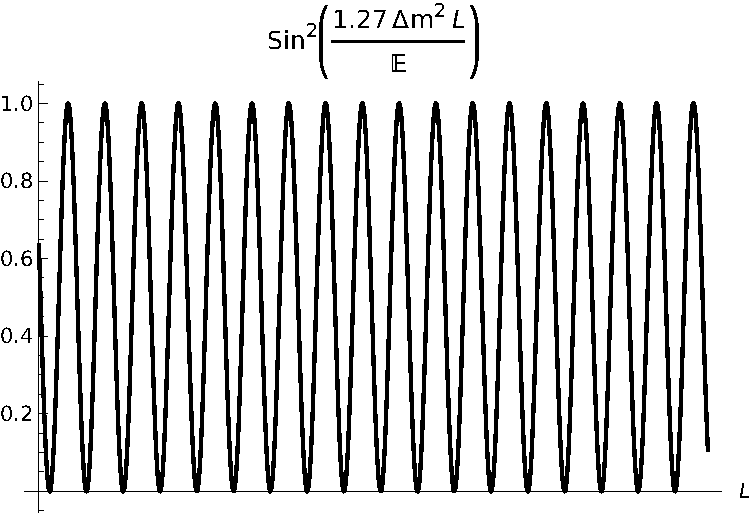
\includegraphics[width=0.75\linewidth]{figures/1.pdf}
	\captionsetup{width=.65\linewidth}
	\caption{%
	This shows a qualitative sketch of $\sin[2](1.27 \Delta m^2 L/E)$, from $L$ to $L+\Delta L$, where $\Delta L$ is the size of the detector.
	In the limit where $\abs{\Delta m}^2 \gg E/L$, the spatial frequency is very high, as depicted by the large number of cycles shown in the graph.
	}
\end{figure}

\section{Large $\Delta m$ Limit}

Since the probability of an oscillation ocurring is
\begin{equation}
	P_{osc}(t) = \sin[2](2\theta) \sin[2](1.27 \Delta m^2\frac{L}{E}),
\end{equation}
the survival probability is just $1-P_{osc}(t)$.
Additionally, for $\abs{\Delta m}^2 \gg E/L$, one can say that the limit of $\sin^2$ goes to the average value of $1/2$.
Thus
\begin{equation}
	2(1-P_{surv}) = \sin[2](2\theta).
\end{equation}
With $P_{surv} = 0.92$, $\sin[2](2\theta) = 0.16$.

\section{Small $\Delta m$ Limit}

In the limit $\abs{\Delta m}^2 \ll E/L$,
\begin{equation}
	\sin[2](1.27 \Delta m^2 \frac{L}{E}) \rightarrow \left(1.27 \Delta m^2 \frac{L}{E}\right)^2.
\end{equation}
Hence
\begin{align}
	1-P_{surv} &= \sin[2](2\theta) \left(1.27 \Delta m^2 \frac{L}{E}\right)^2,\\
	\sin[2](2\theta) &= C \left(\frac{1}{\Delta m^2}\right)^2,
\end{align}
where $C = (1-P_{surv})(E/L)^2$.

\section{The Null result from the CHOOZ experiment}
\subsection{Oscillation Probability}
\begin{align}
	P_{osc} &= \sin[2](2\theta)\sin[2](1.27 \Delta m^2 \frac{L}{E}),\\
	&= 0.085.
\end{align}
\subsection{Allowed or Excluded?}
The point is just barely inside the allowed region, being slightly below the green curve at $\sin[2](2\theta) = 0.1$.

\nocite{*}
\printbib


\stopmcols


\end{document}

